\documentclass[preprint,aps,pra,floatfix]{revtex4-2}

% preamble.tex — shared packages and macros
\usepackage{graphicx}
\usepackage{amsmath,amssymb}
\usepackage{siunitx}
\usepackage{microtype}
\usepackage{xspace}
\usepackage[usenames,dvipsnames]{xcolor}
\usepackage[colorlinks=true,allcolors=blue]{hyperref}

% Abbreviations
\newcommand{\OSL}{osseous spiral lamina\xspace}
\newcommand{\CPS}{canaliculi perforantes of Schuknecht\xspace}
\newcommand{\ST}{scala tympani\xspace}
\newcommand{\SGN}{spiral ganglion neuron\xspace}
\newcommand{\SGNs}{spiral ganglion neurons\xspace}

% Figures path
\graphicspath{{figures/}}

\begin{document}
\title{Toward Living Cochlear Implants: Using Canaliculi Perforantes to Guide Regeneration}
\author{Akihiro J. Matsuoka}\author{Andrew Carpino}\author{Jae Joon Kim}\author{Audrey Meador}\author{Beatriz Nicolau}\author{Gabriela Fortuno}\author{Hudson Liu}\author{Kiersten Russ}\author{Huimin Zhu}\author{Tifany Nguyen}\author{James Friend}
\affiliation{University of California San Diego; Georgetown University School of Medicine; University of California Los Angeles}
\date{\today}
\begin{abstract}
Cochlear implants (CIs) restore hearing by directly stimulating auditory neurons, yet a persistent electrode--neuron gap constrains spatial selectivity and the fidelity of complex listening. This Topical Review outlines a biohybrid approach that leverages the \CPS\ to guide neurites toward recording/stimulation sites while enabling localized therapy.
\end{abstract}
\maketitle
\
\section*{1. Introduction}

Cochlear implants (CIs) are among the most successful neuroprostheses in clinical use, yet their performance plateaus point to a central limitation of contemporary designs: the millimeter-scale distance between stimulating contacts in the \ST and the excitable elements of the auditory nerve within Rosenthal's canal. Even with perimodiolar arrays, this gap attenuates voltage gradients at the target neurons, blurs spatial selectivity through current spread, and limits the fidelity of temporal and spectral cues that underlie speech-in-noise understanding, music perception, and spatial hearing. In short, we have an engineering interface problem at anatomical scale.

This review advances a biohybrid strategy to address that interface. Rather than relying only on closer metallic electrodes or more aggressive scala insertion, we consider how a device can \emph{cooperate} with living tissue to bridge distance and improve coupling over time. The concept is to integrate guidance and regenerative cues into the implant so that neurites from surviving \SGNs can be \emph{recruited} across natural modiolar pathways toward recording/stimulation sites, while the device simultaneously delivers localized therapies and remains surgically practical.

A key anatomical substrate for such an approach is the network of modiolar microchannels historically described as the \CPS. These small perforations in the \OSL and adjacent modiolar bone are implicated in perilymphatic communication and may provide micro-conduits between the \ST and the neural compartments of the modiolus. If patent in adulthood and accessible from the scala, they could be leveraged for controlled delivery (e.g., neurotrophins, enzymes, RNA cargo, extracellular vesicles) and as permissive corridors for guided neurite extension. The hypothesis we explore here is that pairing these intrinsic pathways with appropriately tuned chemical, mechanical, and electrical cues can reduce effective electrode--neuron distance and increase the number of addressable neural elements without resorting to invasive modiolar drilling.

The notion of a ``living'' or biohybrid implant aligns with broader trends in regenerative bioelectronics, where devices are designed to co-integrate with grafted or host tissue to recover function and enable closed-loop control. Recent perspectives argue that such systems will rely on three classes of cues delivered by the interface: (i) chemical (spatiotemporally controlled release of trophic factors, genes, or vesicles), (ii) mechanical (stiffness, roughness, and topography to bias cell behavior and neurite trajectories), and (iii) electrical (fields and stimulation paradigms to modulate migration, growth, and maturation).\citep{CarnicerLombarte2024AdvMat} The cochlea is a stringent proving ground for these ideas because it demands long-term stability in a compact, fluid-filled, delicate environment, with strong constraints on insertion mechanics, biocompatibility, and serviceability.

We also take advantage of recent progress in accelerating the maturation of human stem-cell–derived neurons, which can shorten preclinical timelines and potentially improve the readiness of transplanted or guided cells. In particular, a four-factor small-molecule regimen (``GENtoniK'')---combining an LSD1 inhibitor, a DOT1L inhibitor, an NMDA receptor agonist, and an L-type calcium-channel agonist---has been shown to rapidly increase neuritogenesis, synaptic puncta, and spontaneous firing across multiple human neuron types and in organoids.\citep{Hergenreder2024NatBiotech} While these data are not yet specific to \SGNs, they showcase a generalizable lever to prime human neurons for integration with engineered interfaces. Importantly, subsequent clarification of synaptic current attribution in that work underscores the need for pharmacological validation when interpreting spontaneous postsynaptic events; we keep this caution in view when proposing readouts and benchmarks.

\textbf{Scope and structure.} Section~2 summarizes the epidemiology and economic burden of hearing loss to motivate the need for higher-fidelity interfaces. Section~3 defines the modiolar microanatomy relevant to electrode--neuron coupling and summarizes routes that matter for delivery. Section~4 reviews regenerative evidence across chemical, mechanical, and electrical modalities, highlighting portable findings and limits. Section~5 surveys interface materials and device architectures that can deliver these cues in the cochlea. Section~6 proposes translational benchmarks and constraints, including surgical feasibility and regulatory considerations for combination products. Section~7 closes with a near-term experimental roadmap and open questions.

By consolidating anatomical clarity with actionable interface strategies, we aim to provide a practical scaffold for researchers developing biohybrid approaches to cochlear implantation, and a shared language for otology, neuroengineering, and materials communities working toward the same goal.

\
\section*{2. Epidemiology and Economic Burden of Hearing Loss}

Hearing loss is a major public health concern that affects everyday communication, education, employment, and healthy aging. In the United States, approximately one in eight individuals (13\%, or about 30 million people) aged 12 years and older has measurable hearing loss in both ears, and 15\% of adults (37.5 million) report at least some trouble hearing.\cite{nidcd2021, cdc2010, cdc2021, wilson2014} These figures meet or exceed the prevalence of other common chronic conditions and emphasize the scale at which hearing impairment consumes health system resources and erodes quality of life.

\subsection*{2.1 Prevalence and risk}
Prevalence rises steeply with age and is compounded by cumulative noise exposure and genetic factors. Globally, disabling hearing loss affects a substantial fraction of older adults, with roughly one quarter of those over 60 years affected, while more than one billion young people are estimated to be at risk of noise-induced, permanent hearing loss.\cite{WHO2025} These epidemiologic trends foreshadow increasing demand for accessible hearing care across the life course.

\subsection*{2.2 Direct and indirect economic costs}
The economic burden of hearing loss spans direct medical spending and substantial indirect costs. Direct costs include clinical evaluations, hearing aids (commonly \$1{,}000--\$4{,}000 per pair), cochlear implantation (\$30{,}000--\$100{,}000 per patient), audiologic rehabilitation, speech--language therapy, and ongoing device maintenance. Indirect costs include reduced productivity and employment: adults with hearing loss have higher odds of unemployment (odds ratio \(\approx 1.98\)), and individual annual income losses up to \$30{,}000 have been reported, aggregating to an estimated \$176 billion per year in the U.S.\cite{SocietyCosts2000, Kim2020, Colburn2019, WHO2025} At the global level, the annual societal cost of unaddressed hearing loss was estimated at \$981 billion in 2020, with quality-of-life losses accounting for about 47\% and a majority of costs (\(\sim\)57\%) incurred outside high-income countries.\cite{McDaid2021}

Strategic investment in hearing care is projected to yield substantial returns. The World Health Organization estimates that scaling essential ear and hearing care interventions to 90\% coverage over the next decade would require an additional \$238.8 billion and generate more than \$2 trillion in productivity gains by 2030.\cite{Tordrup2022} From an individual perspective, early cochlear implantation in children can be cost-saving over the life course: one analysis estimated lifetime healthcare costs of \$489{,}274 for a person born with severe-to-profound loss, reduced to \$390{,}931 (95\% CI \$311{,}976--\$471{,}475) when a cochlear implant is provided before 18 months of age, yielding net lifetime savings of \$98{,}343.\cite{Cejas2024}

\subsection*{2.3 Market context and barriers}
The global cochlear implant market was valued at approximately \$2.42 billion in 2023 and is projected to grow to \$6.63 billion by 2034 (compound annual growth rate \(\sim\)9.0\% for 2024--2034).\cite{globenewswire2025cochlear} Demand is driven by aging populations, persistent noise exposure, and recognition of genetic contributions to hearing loss.\cite{WHO2025} Despite demonstrated benefits, the path to cochlear implantation still presents high barriers: total procedure costs often range from \$50{,}000 to \$100{,}000 when all components of care are included, and access can be constrained by insurance coverage, referral patterns, and center availability. The sector includes established manufacturers such as Cochlear Limited (Australia), Advanced Bionics (Sonova Holding AG, Switzerland), Zhejiang Nurotron Biotechnology Co., Ltd. (China), and MED-EL Medical Electronics (Austria). Regulatory requirements for safety and effectiveness---particularly for novel active implantable devices---and the high cost of research and development contribute to significant barriers to entry, while simultaneously creating opportunities for differentiated, high-value innovation.

\subsection*{2.4 Motivation for higher-fidelity, regenerative interfaces}
Taken together, the epidemiologic scale and the economic burden motivate solutions that improve the benefit-to-cost ratio of hearing care. In the context of cochlear implants, narrowing the effective electrode--neuron distance and increasing the number of addressable neural elements are plausible pathways to improved speech-in-noise understanding, music perception, and spatial hearing. These functional gains would be expected to translate into measurable quality-of-life improvements and economic benefits. This review therefore proceeds from population-level need to the anatomical and engineering questions required to enable ``living'' cochlear implants that cooperate with tissue to improve coupling over time.


\section{\label{sec:AnatRationale}Anatomical Rationale}

%%%%%%%%%%%%%%%%%%%%%%%%%%%%%%
%Figure 1 (Beatriz and Humin)
%%%%%%%%%%%%%%%%%%%%%%%%%%%%%%

\begin{figure}[ht]
  \centering
  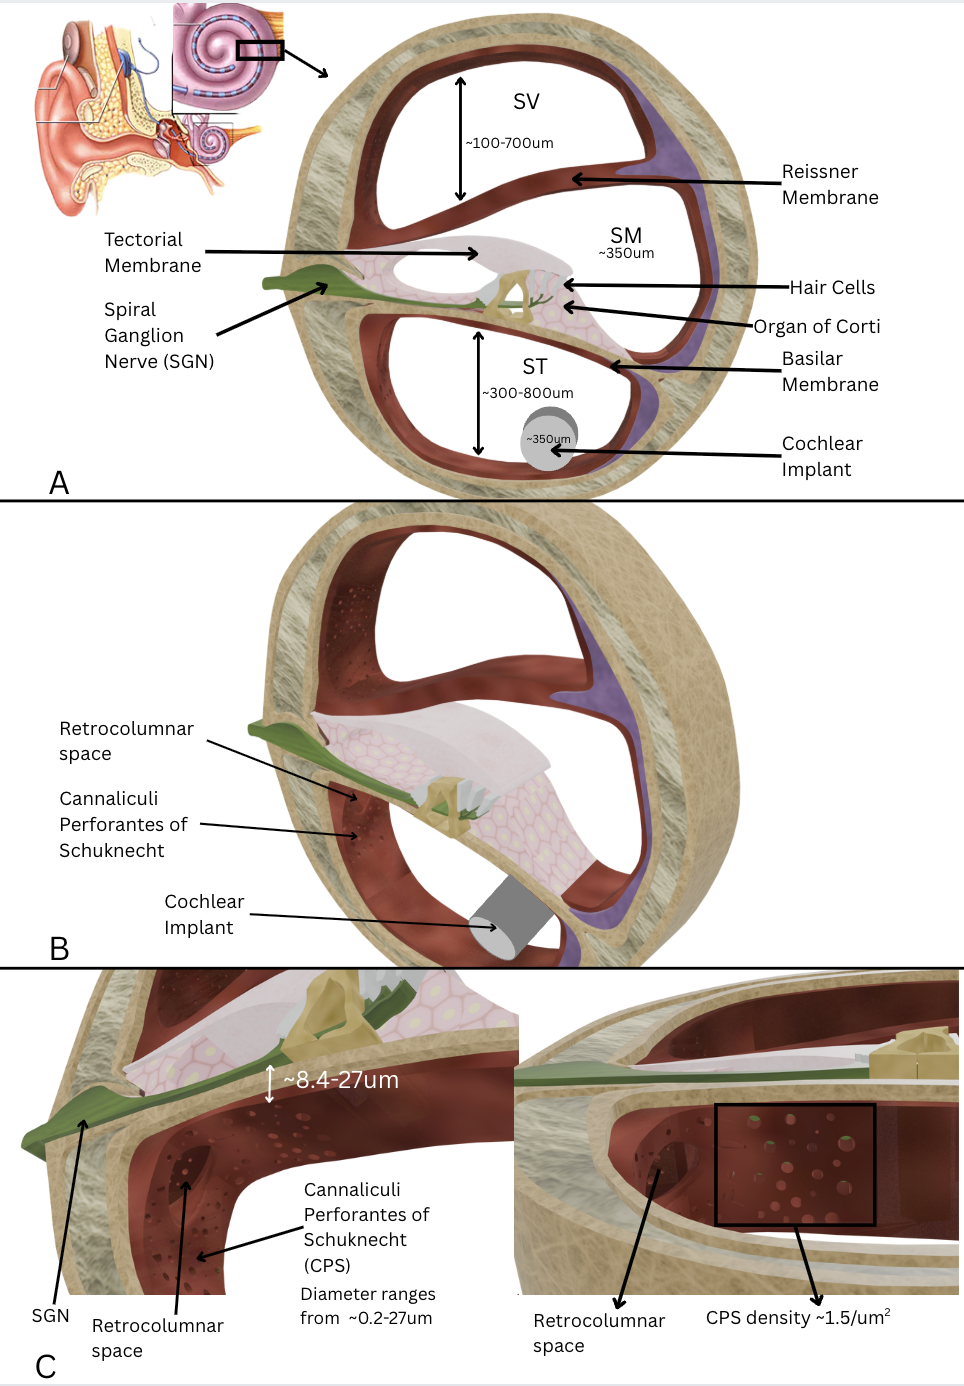
\includegraphics[width=0.8\textwidth]{Figure/3DAnatomyPanel.png}
  \caption{TBW}
  \label{fig:cochlea_overview}
\end{figure}
%%%%%%%%%%%%%%%%%%%%%%%%%%%%%
\subsection{Cochlear scalae in brief}  
The bony labyrinth encloses two perilymph‑filled channels, the \emph{scala vestibuli} and \emph{scala tympani}, which wind around the modiolus and communicate at the helicotrema. Sandwiched between them, the endolymphatic \emph{scala media} houses the organ of Corti on the basilar membrane.  Conventional cochlear implants occupy the scala tympani, placing their contacts within millimeters---but rarely microns---of spiral ganglion neurons (SGNs) embedded in Rosenthal’s canal. Importantly, typical electrode-to-SGN distances are around 0.5–1 mm for modiolus-hugging arrays and up to $\sim1.5-2 mm$ for lateral wall placements \cite{Davis2016}. Even in the best-case scenario, a gap on the order of $10^{2}-10^{3} \mu m$ remains between the electrode and neuron. This physical separation has practical implications: it necessitates current spread through perilymph and bone to reach the neurons, and it underlies why closer electrode positioning (e.g. perimodiolar designs) can reduce stimulation thresholds \cite{Kawano1998}. Furthermore, the distance can vary along the cochlea---apical electrodes often achieve the smallest gaps $\approx0.5 mm$ or less) while mid-cochlear electrodes can be $\approx1 mm$ or more away \cite{Long2014}. These quantitative insights, drawn from human studies, validate that CIs interface with the auditory nerve across a millimeter-scale gulf, rather than forming direct micron-level contact with the neurons. Finally, any natural pores linking the scala tympani to the modiolus are therefore potential highways for drugs, trophic factors, or neurites seeking the electrode array in the scala tympani.


\subsection{Scala Tympani Dimensions and Cochlear Implant feasibility}
\subsubsection{Scala Tympani Anatomy in Humans}
\paragraph{Human[Homo Sapiens]}
:  As briefly mentioned in a previous section, the human scala tympani is a large perilymph-filled canal that narrows from base to apex. Near the basal turn (around the round window region), the ST cross-section is ovoid with a typical vertical height of ~1.2–1.4 mm and width slightly larger \cite{fujiwara2023morphometric}. This corresponds to a cross-sectional area of roughly 2.3 mm² at the base (0°), which then diminishes to about 1.3–1.4 mm² by 180° (half a turn) into the cochlea \cite{fujiwara2023morphometric}. Beyond the basal turn (~360°), the ST lumen becomes more of a flattened triangle in cross-section as it enters the middle and apical turns. The height drops below 1 mm in the upper turns, and the area continues tapering (often $<$ 1 mm² near the apex). Thus, the basal ST can accommodate larger diameters, whereas the apical region is very small and slit-like. Notably, the ST width is consistently greater than its height at any given point \cite{hatsushika1990dimensions}, reflecting the elongated shape of the duct. The human cochlea is ~35–36 mm in uncoiled length (2.5–2.7 turns) and the total ST volume is about 29 $\mu$L \cite{Liu2023FEA}.

\subsection{Canaliculi Perforantes of Schuknecht (CPS)}  
Schuknecht’s original temporal‑bone study (1959) revealed hundreds of microscopic channels piercing the osseous spiral lamina (OSL) from the scala tympani toward the modiolus \cite{schuknecht1959}.  Later histology and scanning‑electron microscopy confirmed that these \textit{canaliculi perforantes} concentrate along the modiolar plate, especially in the basal and middle turns \cite{Schuknecht1963,lim1970,sando1971,masuda1971,tanaka1973}. The CPS are predominantly located on the scala tympani surface of the OSL, in the lower (inferior) bony lamina that underlies the basilar membrane. They are especially numerous in the modiolar (medial) region of the OSL, adjacent to the modiolus where the SGNs are housed \cite{shepherd2004}. Human CPS lumina were measured from 0.2 to 23 $\mu$ m against an OSL thickness that tapers from 26.8 $\mu$ m basally to 8.4 $\mu$ m apically \cite{shepherd2004}.  These dimensions overlap both the caliber of regenerating SGN neurites and the 10--30 $\mu$ m diffusion length of neurotrophins such as NT‑3 or BDNF in perilymph, making each pore a matched conduit for axonal ingress and trophic support.

\subsection{Other modiolar communication routes}  
\begin{enumerate}
\item Trabecular Meshwork: Rask‑Andersen and colleagues identified additional “trabecular meshwork” apertures—up to 100 $\mu$m in the scala vestibuli and 40 $\mu$ m in the scala tympani—plus fenestrations along perivascular and perineural sheaths \cite{raskandersen2006}.  Together with the CPS, they form a porous continuum that contradicts the notion of an impervious modiolar wall, permitting pressure equilibration and macromolecular traffic between perilymph and the SGN somata \cite{raskandersen2006, shepherd2004}.

\item Larger Modiolar Vascular Outlets: In addition, they identified "larger modiolar vascular outlets" as larger openings (up to $\sim$100 $\mu$m) adjacent to the anterior and posterior spiral modiolar veins and arteries, whose function is to permit exchange between perilymph and perivascular spaces, contributing to perilymph homeostasis and potential drug delivery routes. Finally, "mesothelial cell–covered fenestrae" was defined as thin cellular sheets ($<$ 3 $\mu$m) lining the OSL and modiolar surface, interspersed with micropores (up to $\sim$ 40 $\mu$m) on both the scala tympani and scala vestibuli sides. The function of mesothelial cell-covered fenestrae is to provide semi-permeable lining over the bony channels, allowing diffusion of small and large molecules while maintaining fluid compartmentalization \cite{raskandersen2006, shepherd2004}.

\item Mesothelial Cell–Covered Fenestrae: Thin cellular sheets ($<$ 3 $\mu$m) lining the OSL and modiolar surface, interspersed with micropores (up to $\sim$40 $\mu$m) on both the scala tympani and scala vestibuli sides. Mesothelial cell–covered fenestrae allows for exchange between perilymph and perivascular spaces, contributing to perilymph homeostasis and potential drug delivery routes \cite{raskandersen2006, shepherd2004}.

\end{enumerate}

\begin{table}[ht]
\centering
\caption{Quantitative dimensions of perilymph–modiolar passage channels in the basal turn of the human cochlea}
\label{tab:channels_dimensions}
\begin{tabular}{lll}
\toprule
\textbf{Structure / Channel} & \textbf{Dimension (basal turn)} & \textbf{Source} \\
\midrule
Canaliculi Perforantes Schuknecht (CPS) & Mean diameter $5.2 \pm 4.9\ \mu$m (range 0.2--23.0 $\mu$m)       & \cite{ShepherdColreavy2004} \\
Osseous spiral lamina (OSL) thickness & $26.8 \pm 6.0\ \mu$m                                      & \cite{ShepherdColreavy2004} \\
Density of canaliculi (pores/$\mu$m²)   & $1.05 \pm 1.03$ pores/$\mu$m²                                  & \cite{ShepherdColreavy2004} \\
Mesothelial cell–sheet thickness    & $0.3$--$3\ \mu$m                                            & \cite{raskandersen2006} \\
Trabecular‐mesh “fenestrae” size    & Up to $\sim 40\ \mu$m (holes in modiolar wall)             & \cite{raskandersen2006} \\
Modiolar vascular outlets           & Pores up to $\sim 100\ \mu$m                               & \cite{raskandersen2006} \\
\bottomrule
\end{tabular}
\end{table}

\subsection{Functional Pathways and SGN Connectivity Through CPS}
The CPS form a network of microscopic pores through the OSL that directly links the fluid of the scala tympani with the perimodiolar spaces in Rosenthal’s canal \cite{raskandersen2006}. By puncturing the lower plate of the OSL---alongside gaps in its mesothelial lining---and opening into the retrocolumnar trabecular meshwork and perivascular channels of the modiolus, these tiny canals create a continuous perilymphatic pathway from the ST into the SGNs. As a result, the extracellular fluid bathing the SGN cell bodies is essentially the same perilymph that fills the scala tympani, permitting free interchange of ions, nutrients, signaling molecules, and even therapeutic agents or pathogens between these compartments.

Although the true nerve fiber bundles use larger foramina (habenula perforata and modiolar conduits) to enter and exit Rosenthal’s canal, the canaliculi perforantes run alongside and between those fiber routes, serving as perineural and perivascular fluid conduits. Glueckert et al. found nerve fibers in BDNF-treated animals that progressed into CPS. These fibers reveal a myelin layer close to the OSL and within the bony canaliculi but with extreme swelling when entering the scala typani \cite{glueckert2008}. Li et al. also observed SGN neurites projecting across the OSL wall into the ST through the CPS \cite{Li2017}. Similar observations have been reported by others \cite{Staecker1996, Leake2008, Leake2011, Wise2011}.  

\subsection{Distance Between Cochlear Implant Electrodes and Spiral Ganglion Neurons in Rosenthal’s Canal}
Conventional CI electrode arrays reside in the scala tympani and thus are separated from the SGNs in Rosenthal’s canal by the bony modiolus. Multiple anatomical and imaging studies confirm that across patients and electrode positions, the distance between an electrode contact and the SGNs in Rosenthal’s canal generally spans from a few hundred microns up to $\sim$1–2 mm. A detailed CT scan study of perimodiolar arrays reported a total range of $\sim$0.1 mm up to 1.8 mm in electrode-to-modiolus separation \cite{Long2014}. Histological section measurements estimate that in the human basal turn, a lateral-wall electrode may be roughly $\sim$2 mm away from the spiral ganglion (by radial distance). These data support the statement that CI contacts lie within millimeters—but rarely mere microns—of the SGNs\cite{Schmidbauer2023}.

The electrode-to-SGN distance is not uniform along the cochlea; it varies with the cochlear turn and electrode position. Overall, the closest electrode-neuron proximities are achieved in the apical cochlea, with mid-cochlea generally the farthest on average, though patient-specific anatomy causes considerable variability (overall 0.1--1.8 mm range in the cited study) \cite{Long2014}.

\subsection{The Electrode-Neuron Gap Does Matter}
Kawano et al. (1998) performed detailed histopathologic exams of five human cochleae with CIs and measured the distance between each electrode band and the center of Rosenthal’s canal \cite{Kawano1998}. They reported that these electrode-to-SGN distances were in the millimeter range, and importantly found a correlation between greater distance and higher electrical thresholds and comfort levels. In other words, electrodes that sat farther (several millimeters) from the SGNs required more current to evoke hearing, reinforcing that distance is a key factor. The same study noted that intracochlear fibrosis or new bone formation could increase the electrode-modiolus distance, sometimes pushing contacts farther than their design intends. Nadol and colleagues, in histopathologic surveys, likewise estimated distances on the order of 0.5–2 mm and observed that any translocation of an array out of scala tympani (or trauma to the modiolus) can reduce SGN counts, further emphasizing that the electrode-neuron gap matters \cite{nadol1990,Nadol1989}. Computational models and anatomic maps further illustrate these distances. For example, a recent finite-element model by Sriperumbudur et al. (2024) examined electrical stimulation with a perimodiolar CI and assumed a ~0.3 mm gap between the electrode and modiolus as a typical design. This value (300 $\mu$ m) was chosen to reflect a snug perimodiolar placement, yet it still highlights that even in simulation the contacts are not assumed to be touching the neurons (a 0.3 mm gap leaves space for the bony wall and perilymph) \cite{Sriperumbudur2024}. 

\subsection{Surgical implications for biohybrid CIs}  
Because CPS density peaks in the basal OSL, traumatic insertion or aggressive drilling in this region risks sealing the very pathways that a biohybrid implant aims to exploit \cite{shepherd2004}.  Conversely, electrodes engineered with microfluidic ports or neurotrophin‑releasing sleeves could harness these pores to establish steep radial gradients that attract transplanted or residual neurites toward the contacts.  Designing arrays that spare, rather than violate, the CPS therefore becomes as important as thread depth, pitch, or perimodiolar curl.  Leveraging these natural conduits should reduce reliance on bulk diffusion, localize therapy to the modiolus, and ultimately tighten the electrode–neuron interface—a prerequisite for the stem‑cell and material strategies developed in the following sections. Future biohybrid implants are expected to incorporate microfluidic drug delivery (e.g., convection‑enhanced or electrically driven release) to steer regeneration locally within the cochlea \cite{Carnicer-Lombarte:2025aa}.


\section*{4. Stem-cell–derived assembloids and hydrogel scaffolds for a living cochlear implant}

\noindent
Biohybrid cochlear implant concepts rely on living neural elements that can mature, respond to therapy, and form or re-form synapses with host targets. In practice this means (i) supplying the \emph{right cells} in the \emph{right microenvironment} and (ii) coupling them to the device through a mechanically and electrochemically compatible interface. In this section we outline why three-dimensional (3D) stem-cell constructs---from simple spheroids to complex \emph{assembloids}---are preferred over dissociated cultures, and how xeno-free hydrogels can provide a cochlea-ready niche that also supports localized delivery and chronic electrical interfacing.

\subsection*{4.1 Why 3D? From spheroids to organoids to assembloids}
Dissociated, two-dimensional SGN cultures show fragile survival and limited maturation, whereas 3D environments provide a pro-survival, pro-maturation niche with improved neuritogenesis, synaptic puncta, and electrophysiological properties closer to native SGNs.\citep{Zine2021StemCells,Sun2023CellProlif,Koehler2017NatBiotech} Spheroids (single- or few-lineage aggregates) are easy to form and improve retention and trophic support after transplantation relative to single-cell suspensions.\citep{Chang2020ActaBiomaterialia} Inner-ear \emph{organoids} add rudimentary cyto-architecture and hair-cell--to--SGN ribbon synapses.\citep{Koehler2013Nature,Koehler2017NatBiotech,Sun2023CellProlif} 

\emph{Assembloids} intentionally combine multiple, precisely chosen cell lineages to recreate elements of the SGN microenvironment---for example SGNs with Schwann cells, satellite glia, and a microvascular compartment---achieving myelination, robust trophic support, and more mature firing phenotypes than neuron-only constructs.\citep{Xia2023StemCellReports,Oliveira2023FrontiersPN} Where hair cells are not required for the intended biohybrid function, assembloids can omit them to reduce complexity while retaining essential SC/vascular support. Emerging small-molecule maturation regimens (e.g., “GENtoniK”) can further accelerate human neuron maturation in 3D systems; when used, these require pharmacological validation of synaptic readouts and careful dose scheduling to maintain viability and lineage identity.\citep{Hergenreder2024NatBiotech}

\subsection*{4.2 Design of SGN assembloids: cell composition and roles}
A practical SGN assembloid includes five components whose functions are complementary: (i) \textbf{SGNs} (afferent neurons, the principal excitable elements); (ii) \textbf{Schwann cells} (myelination distal to the habenula; metabolic and trophic support; debris clearance; immune orchestration);\citep{Oliveira2023FrontiersPN,Moss2024iScience} (iii) \textbf{satellite glia} (ion and neurotransmitter homeostasis around somata); (iv) \textbf{microvascular cells} (endothelial cells and pericytes to resist diffusion limits and enable sustained trophic flux); and (v) \textbf{fibroblast/perineurial cells} (ECM deposition and compartmental definition). Co-culture in 3D favors compact myelin formation around peripheral axons and higher-amplitude/phase-locked firing, with evidence of ribbon synapses in innervated cochlear organoid systems.\citep{Xia2023StemCellReports}

\subsection*{4.3 Hydrogel scaffolds as the SGN niche}
The cochlea imposes stringent constraints on materials: (i) mechanical compliance in the low-kPa regime to avoid disturbing micromechanics; (ii) permeability for oxygen, ions, and macromolecules; (iii) xeno-free chemistry for translation; (iv) acoustic compatibility; and (v) processability for minimally invasive delivery. Several animal-free hydrogels meet these needs to different degrees:

\begin{itemize}
	\item \textbf{VitroGel\textsuperscript{\textregistered} NEURON}: shear-thinning, self-healing polysaccharide network with customizable peptide motifs; $E \approx 0.5$--$2$ kPa; rapid recovery; excellent for low-attenuation acoustic environments.\citep{Zine2021StemCells}
	\item \textbf{PeptiGel\textsuperscript{\textregistered} $\alpha 4$}: self-assembling $\beta$-sheet peptide with intrinsic RGD/IKVAV motifs; transparent; GMP-compatible; $E \approx 1$--$3$ kPa.\citep{Millesi2023ACSAMI}
	\item \textbf{PuraMatrix\textsuperscript{\textregistered} (RADA16)}: very soft nanofibrillar network ($E \approx 0.1$--$1$ kPa); highly hydrated; may micro-collapse without reinforcement.\citep{Zhong2010NNR}
	\item \textbf{RGD–alginate}: enzymatically degradable, Ca$^{2+}$-crosslinked hydrogel; tunable but can gel rapidly and reach higher stiffness ($3$--$20$ kPa) unless crosslinking is carefully limited.\citep{Mooney2011TEA}
	\item \textbf{HyStem-HP}: thiolated hyaluronic acid + gelatin + PEGDA; heparin-binding for sustained neurotrophin delivery; workable but short handling window ($\sim$5 min).\citep{Zhong2010NNR}
	\item \textbf{PEG–DA (photopolymerized)}: highly tunable elastic modulus ($0.5$--$20$ kPa); chemically inert and acoustically acceptable only at low crosslink density; requires RGD/ECM grafting for SGN adhesion.\citep{Mooney2011TEA}
\end{itemize}

A minimal design rule emerges: choose a \emph{xeno-free, soft (0.5--3 kPa), peptide-adhesive} gel that can be injected and quickly recover, then decorate with ECM motifs (RGD/IKVAV/YIGSR) and gradients of neurotrophins (e.g., BDNF/NT-3) to bias neurite trajectories. In several cochlear and neural contexts, peptide-functionalized hydrogels attract SGN neurites and support long-term survival; in inner-ear models, nanofibrillar cellulose and related systems have been used to create a 3D niche with \emph{sustained} factor release.\citep{Pancratov2017ColSurfB,Chang2020ActaBiomaterialia}

\subsection*{4.4 Coupling assembloids to the implant: conductive and anti-fouling interfaces}
Hydrogels can be rendered conductive or used as drug-eluting sleeves on perimodiolar arrays to narrow the electrode--neuron gap while improving chronic electrochemistry.\citep{Dalrymple2020JNE,Chikar2012Biomaterials} Composite gels (e.g., GelMA/PEG blended with PEDOT:PSS) can enhance charge transfer and, in vitro, protect cochlear epithelia from oxidative stress.\citep{Tan2024Biomolecules} In parallel, photografted \emph{zwitterionic} hydrogel coatings on commercial CI materials reduce the foreign body response and fibrosis in vivo, improving the long-term interface for both recording and stimulation.\citep{Horne2023ActaBiomaterialia} 

\subsection*{4.5 Integration with modiolar microchannels and localized delivery}
When positioned along the medial face of a perimodiolar array, an assembloid-bearing hydrogel sleeve can interface with the modiolar surface and potentially leverage canaliculi perforantes (CPS) as micro-conduits for neurite entry and factor exchange (see Sec.~3). A heparinized or nanoporous formulation enables \emph{slow release} of BDNF/NT-3 analogues or RNA cargo at the scala–modiolus boundary, sustaining trophic gradients without repeated infusions.\citep{Chikar2012Biomaterials,Johansen2018PLoSOne,StPeter2022FrontBioeng} Micro-topography on the adjacent polymer shank can further bias growth cone trajectories to the intended stimulation sites, allowing chemical and physical guidance to act in concert.\citep{Truong2021HearRes,Vecchi2024JNE}

\subsection*{4.6 Readouts and benchmarks}
For assembloid–hydrogel systems, we recommend separating \emph{proof of integration} from \emph{performance} claims:
\begin{enumerate}
	\item \textbf{Survival and maturation:} viability and myelination $\geq$8~weeks; expression of SGN subtype markers; firing rate stability under repeated stimulation.\citep{Xia2023StemCellReports,Moss2024iScience}
	\item \textbf{Synaptic measures:} ribbon synapse counts and synaptic protein puncta; pharmacological validation of spontaneous postsynaptic events in 3D cultures.\citep{Hergenreder2024NatBiotech}
	\item \textbf{Guidance efficacy:} fraction of neurites traversing toward the modiolar side and into CPS-accessible zones under defined gradients/topographies.\citep{Truong2021HearRes,Vecchi2024JNE}
	\item \textbf{Electrode coupling:} impedance/phase angle and charge storage capacity with conductive gel coatings versus bare contacts under accelerated soak and stimulation.
	\item \textbf{Tissue response:} fibrosis thickness and macrophage phenotype around coated versus uncoated leads in relevant animal models.\citep{Horne2023ActaBiomaterialia,Fibranz2025JFB}
\end{enumerate}

\subsection*{4.7 Translational notes}
To preserve clinical workflow, the construct should be injectable, self-healing, and visible (e.g., via MR-compatible contrast or OCT) during and after insertion. For regulatory alignment, choose xeno-free chemistries with available GMP lots; minimize persistent animal proteins (e.g., Matrigel, gelatin) unless justified by benefit–risk; and document sterilization compatibility and shelf stability. Acoustic/mechanical testing in saline at body temperature is essential to ensure that the hydrogel sleeve does not degrade micromechanics or increase attenuation in the basal turn.

\medskip
\noindent\textbf{Summary.} Human stem-cell–derived SGN assembloids offer a controllable, multi-lineage route to a living CI interface, while modern, xeno-free hydrogels supply the compliant, bioactive niche and delivery vehicle those cells need. When combined with conductive and anti-fouling coatings, these materials can narrow the effective electrode–neuron distance and maintain implant performance while enabling regeneration-driven improvements over time.

\section{Biomaterial interfaces for next‑generation cochlear implants}
\label{sec:biomaterials}

Biohybrid cochlear implants must balance three coupled demands: (i) efficient charge transfer at the metal–tissue boundary, (ii) mechanical and electrochemical compliance to match inner‑ear tissues while maintaining stable stimulation and recording, and (iii) durable resistance to fibrosis, infection, and biofouling. A practical material stack proceeds from established noble‑metal contacts to conductive polymer interlayers, then to conductive hydrogels and anti‑fouling chemistries that enable regenerative and drug‑delivery functions \cite{CarnicerLombarte2024AdvMat}.

\subsection{Platinum–iridium: the clinical baseline}
Platinum–iridium (Pt–Ir) remains the workhorse for intracochlear electrodes due to corrosion resistance and long clinical track records. Chronic stimulation studies continue to refine safe operating windows and dissolution limits, and thin‑film variants have been characterized electrochemically and in vivo \cite{Shepherd2020,Dalrymple2020_ptir}. Pt–Ir establishes a reliable, inert foundation but offers limited mechanical compliance and comparatively modest charge‑injection capacity relative to newer coatings.

\subsection{Conductive polymers (CPs)}
Conductive polymers such as PEDOT:PSS and polypyrrole (PPy) lower impedance and increase charge‑injection capacity over bare Pt–Ir, improving the efficiency of neural interfaces \cite{Venkatraman2011-ql,li2025pedot}. PEDOT and PPy coatings can be patterned or covalently anchored to metals to enhance adhesion and water stability \cite{Kleber2017,Chhin2018}. Beyond electrochemistry, CPs have served as drug/growth‑factor reservoirs at the cochlear interface—for example, PPy matrices loaded with NT‑3 or BDNF promoted neurite outgrowth from auditory neurons in preclinical models \cite{Richardson2007,Richardson2009,Evans2009-cm}. Overall, CPs are a mature route to reduce impedance and introduce biomolecule functionality, though long‑term cohesion and delamination under intracochlear micromotion remain design concerns \cite{li2025pedot}.

\subsection{Conductive hydrogels (CHs)}
Conductive hydrogels combine soft, tissue‑like mechanics with ionic/electronic transport, further reducing interfacial impedance while improving conformal contact with the modiolar wall \cite{Green2012}. In cochlear and related neural contexts, CH coatings improved electrochemical performance and chronic stability under stimulation \cite{Hassarati2014,Dalrymple2020,Hyakumura2021}. Practical integration typically uses a thin CP “tie‑layer” (e.g., PEDOT) or surface roughening/priming to secure the hydrogel mechanically and chemically to the metal contact \cite{Kleber2017,Chhin2018}. Because the hydrogel phase can host cargos, CHs are attractive vehicles for anti‑inflammatory agents and neurotrophins at the electrode–neuron interface \cite{Green2012,Hassarati2014}.

\subsection{Structural carriers and drug depots}
A compliant structural sheath can buffer insertion forces and serve as a long‑lived drug reservoir. Poly($\varepsilon$‑caprolactone) (PCL) is a representative, FDA‑cleared polyester used broadly for neural and ocular drug delivery; its slow hydrolysis and tunable porosity enable weeks‑to‑months release without acidic byproducts \cite{Boia2019,Zhou2018}. In a biohybrid CI context, a thin porous PCL layer can house neurotrophins or small molecules while preserving overall array flexibility.

\subsection{Anti‑fouling and anti‑inflammatory surface chemistries}
Surface chemistries that resist protein adsorption and cellular adhesion are increasingly being applied to CI carriers. Photografted zwitterionic hydrogels on clinical silicone carriers reduced the foreign‑body response \textit{in vivo}, supporting their translational relevance for the cochlea \cite{Horne2023}. In parallel, steroid‑eluting arrays (dexamethasone) have advanced from preclinical to clinical evaluation, with studies reporting reduced impedances and inflammatory markers and ongoing assessments of hearing preservation and safety \cite{Kiefer2008Dexameth,Briggs2020,xu2018,Rahman2024,Toulemonde2021}. Together, anti‑fouling and controlled‑release strategies complement CP/CH stacks by modulating the host response over the critical peri‑implant period.

\subsection{Sustained neurotrophin delivery and neurite guidance}
A recurring theme in auditory‑nerve protection and re‑innervation is the sustained, spatially controlled presentation of BDNF/NT‑3 to spiral ganglion neurons (SGNs). Multiple preclinical studies show that local BDNF delivery enhances SGN survival and neurite extension toward electrodes; CPs, CHs, and cell‑based depots have been explored as vehicles \cite{Evans2009-cm,Chikar2012,Leake2013,Scheper2019}. When combined with microanatomical pathways (e.g., modiolar microchannels described earlier) and compliant electrode coatings, these delivery systems could help narrow the electrode–neuron gap.

\subsection{Model‑informed design}
Finite‑element and transport modeling can help set realistic concentration windows, release durations, and spatial gradients that attract neurites without off‑target effects. Recent inner‑ear models explicitly optimize neurotrophin gradients to bridge the electrode–neuron distance and can be aligned with emerging regulatory guidance for in‑silico evidence \cite{Nella2022NeurotrophinGradients,Zhang2023CFD,USFDA2021InSilico}. Modeling also supports the engineering of integrated arrays that combine stimulation, drug delivery, and compliance \cite{Borenstein2011,Lenarz2020FirstHuman}.

\paragraph{Design rules at a glance.}
\emph{Baseline:} Pt–Ir contacts for durability \cite{Shepherd2020,Dalrymple2020_ptir}. 
\emph{Impedance and charge injection:} add PEDOT/PPy where stable adhesion can be ensured \cite{Venkatraman2011-ql,li2025pedot,Chhin2018}. 
\emph{Compliance and cargo:} overlay with a conductive hydrogel for soft contact and local delivery \cite{Green2012,Hassarati2014,Dalrymple2020}. 
\emph{Host response:} graft anti‑fouling (e.g., zwitterionic) layers and/or incorporate anti‑inflammatories \cite{Horne2023,Kiefer2008Dexameth,Briggs2020}. 
\emph{Regeneration:} embed sustained neurotrophin sources and use model‑guided gradients \cite{Evans2009-cm,Leake2013,Nella2022NeurotrophinGradients}. 
\emph{Perspective:} these choices align with broader trends in biohybrid regenerative bioelectronics \cite{CarnicerLombarte2024AdvMat,Hergenreder2024NatBiotech}.

\section{Surface Modifications to Enhance Neuron--Electrode Interactions}
\label{sec:surface_mods}

A persistent barrier to cochlear implant (CI) performance is the micrometer–millimeter gap between the electrode surface and spiral ganglion neurons (SGNs), which forces large current spread and degrades channel selectivity. In a biohybrid CI, surface engineering can be used to (i) lower the electrochemical barrier at the interface, (ii) physically guide neurites toward the contacts, and (iii) suppress the early protein fouling and chronic inflammatory cascades that otherwise raise impedance and reduce neural proximity. Below we outline four complementary approaches and design considerations for integrating them into a unified, regeneration‑supportive interface.

\subsection{Approach 1: Microstructured Electrode Surfaces}
Microscale topography can bias SGN neurite alignment and extend the effective “capture radius” of the contact. Repeating ridge–groove patterns (periods $\sim$5–20\,\textmu m; depths $\sim$1–5\,\textmu m) consistently increase neurite alignment along the pattern axis and improve turning fidelity at corners, effects attributed to growth‑cone mechanosensation and downstream calcium signaling \cite{Wang2013,Chen2014}. In vivo, microgrooved CI electrodes show the expected trade‑off: improved neurite guidance and interface stability must be balanced against insertion trauma if protruding features are too tall or sharp \cite{Lee2019}. Practical guidance is to keep features shallow and rounded, blend them into a compliant coating (below), and co‑present permissive ECM ligands where appropriate (e.g., laminin stripes) to amplify topographic bias without adding stiffness discontinuities at the leading edge \cite{Evans2007LamininFibronectin,Vega1995LamininCollagenIV}.

\subsection{Approach 2: Conductive and Electroactive Coatings}
Roughened noble metals and electroactive polymers reduce interfacial impedance and increase charge‑injection capacity. PEDOT and polypyrrole (PPy) films, including interpenetrating PEDOT–hydrogel networks, produce large, stable impedance reductions and better charge transfer under chronic stimulation \cite{Venkatraman2011-ql,Goding2017,Dalrymple2020,ABIDIAN20081273}. Biofunctionalization of these films (e.g., RGD‑ or peptide‑modified PEDOT; drug‑loaded PPy) further supports cell adhesion and controlled factor release directly from the electrode surface \cite{Chikar2012}. For a biohybrid stack, a thin PEDOT (stability) over PPy (loading) can sit beneath a soft, conductive hydrogel to match tissue modulus while preserving low impedance and space for embedded trophic depots (Section~\ref{sec:materials_stack}, if used). Key checks are adhesion under accelerated aging, charge density limits in saline that mimic perilymph, and retention of low noise after sterilization \cite{Venkatraman2011-ql,Dalrymple2020}.

\subsection{Approach 3: Antimicrobial and Pro‑healing Interfaces}
Early bacterial colonization and the ensuing foreign‑body response are major risks for any chronic implant. Polydopamine (PDA) is a versatile primer that improves coating adhesion and can present bioactive peptides; on silicone CI carriers, PDA–peptide films increase cell adhesion and viability \cite{Schendzielorz2017}. Zwitterionic chemistries (e.g., sulfobetaines) grafted or deposited onto CI materials markedly reduce nonspecific protein adsorption and leukocyte adhesion, lowering inflammation in vivo and improving stability at the electrode–tissue interface \cite{Horne2023,Chen2023-ba}. Complementary strategies include antioxidant/antibiofilm polysiloxane coatings (e.g., N‑acetyl‑L‑cysteine–modified siloxanes) that inhibit biofilm formation while maintaining polymer stability under physiological conditions \cite{Cozma2021-jb}. In a layered design, these chemistries can be placed as the outermost surface (tissue‑facing) while leaving the underlying electroactive layers to handle charge transfer.

\subsection{Approach 4: Anti‑fouling and Anti‑biofilm Surface Chemistry}
Hydration‑rich, charge‑balanced surfaces (zwitterions; highly hydrophilic brushes) resist the protein conditioning film that otherwise seeds fibroblast/macrophage recruitment and biofilm growth. Recent zwitterion‑modified CI materials showed large reductions in postoperative infection and inflammatory cell adhesion, with preservation of low impedances relative to unmodified controls \cite{Chen2023-ba,Horne2023}. When antimicrobial action is required (e.g., revision or high‑risk cases), chemistries that provide sustained bactericidal activity without cytotoxicity to SGNs are preferred; NAC‑functional polysiloxanes are one such route compatible with elastomeric carriers \cite{Cozma2021-jb}. These layers should be validated for (i) stability under electrical pulsing, (ii) sterilization compatibility, and (iii) retention of anti‑fouling function after mechanical insertion testing.

\paragraph{Design guidance (summary).}
\begin{itemize}
	\item \textbf{Start with impedance and modulus:} pair a stable electroactive coating (PEDOT $\pm$ PPy) with a compliant conductive hydrogel to lower $Z$ and match cochlear tissue stiffness \cite{Venkatraman2011-ql,Goding2017,Dalrymple2020}.
	\item \textbf{Add gentle topography for guidance:} shallow ($\lesssim$2--3\,\textmu m) ridges/grooves aligned to the longitudinal axis can bias neurite extension without adding insertion risk \cite{Wang2013,Chen2014,Lee2019}.
	\item \textbf{Cap with anti‑fouling chemistry:} use zwitterionic or PDA‑primed, zwitterion‑grafted layers as the tissue‑facing surface; add targeted antimicrobial/antioxidant functionality if clinically indicated \cite{Horne2023,Chen2023-ba,Cozma2021-jb,Schendzielorz2017}.
	\item \textbf{Co‑design with biochemical release:} where trophic support is provided (e.g., BDNF depots described earlier), align microtopography with release gradients to steer neurites toward contacts while maintaining low impedance \cite{Chikar2012,Goding2017}.
\end{itemize}
Taken together, these surface modifications provide a practical path to shrink the functional electrode–neuron gap and stabilize the interface over time—both prerequisites for any biohybrid CI that aims to recover finer spectral resolution.

\section{Surface-Acoustic-Wave (SAW) Acoustofluidics for Biohybrid Cochlear Implants}
\label{sec7}

\noindent\textbf{Why SAW for the cochlea?} Surface-acoustic-wave (SAW) devices localize acoustic energy within a few micrometres of a piezoelectric surface, enabling contactless manipulation of liquids and cells at power densities appropriate for microfluidics.\cite{Ding2013,rufo2022} For a biohybrid CI, this offers three review-level advantages: (i) on‑demand transport and mixing of tiny payloads (neurotrophins, vesicles, or cell spheroids) near the electrode–tissue interface, (ii) non‑contact patterning that can preserve delicate neurites and support cells, and (iii) the possibility of co‑integrated label‑free biosensing using SAW resonators.\cite{Agostini2021_UHFSAW,Mandal2022}

\paragraph{Operating regimes and substrates.} Conventional SAW microfluidics drives interdigitated transducers (IDTs) at tens to hundreds of megahertz on high‑coupling substrates (e.g., 128$^{\circ}$ YX‑LiNbO$_3$ or sputtered AlN/ZnO on glass), producing acoustic streaming and radiation forces that move particles and shape flows at the microscale.\cite{Ding2013,Campbell1998} At still higher frequencies, ultra‑high‑frequency SAW (UHF‑SAW; $\sim$300~MHz–3~GHz) increases surface confinement and mass‑loading sensitivity, which is advantageous for compact biosensors.\cite{Agostini2021_UHFSAW} These regimes are all compatible in principle with thin, flexible form factors required in the inner ear.

\paragraph{What SAW can \emph{do} in this context (evidence base).}
\begin{itemize}
	\item \emph{Microtransport and gradient formation.} SAW streaming and oscillating microbubbles can generate stable, tunable chemical gradients (tens to hundreds of microns) suitable for guiding neurite outgrowth or dosing cells adhered near contacts.\cite{Ahmed2016_LabChip,Ding2013}
	\item \emph{Cell handling and patterning.} SAW fields can seed, trap, and arrange cells and multicellular aggregates (spheroids/organoids) with high viability, supporting the assembly of structured co‑cultures without direct contact.\cite{Li2007,rufo2022} For a biohybrid CI, this suggests a route to position iPSC‑derived SGN spheroids or Schwann‑cell–neuron co‑aggregates adjacent to electrodes.
	\item \emph{Sensing.} SAW resonators provide label‑free, real‑time readouts of adsorbed mass and viscoelastic changes, enabling detection of proteins or vesicles and potentially monitoring drug‑release kinetics at the electrode surface.\cite{Agostini2021_UHFSAW,Mandal2022}
\end{itemize}

\paragraph{Relevance to cochlear microanatomy.} As reviewed in Section~\ref{sec:cps}, the Canaliculi Perforantes of Schuknecht (CPS) form micron‑scale passages between the scala tympani and perimodiolar spaces.\footnote{We refer the reader to Section~\ref{sec:cps} for CPS dimensions and continuity with perimodiolar fluid spaces.} SAW‑generated microflows or gradients could, in principle, be shaped to concentrate factors toward CPS‑rich zones along the osseous spiral lamina, complementing diffusion‑based strategies by adding spatiotemporal control at sub‑millimetre length scales.\cite{Ding2013,Ahmed2016_LabChip}

\paragraph{Integration constraints (review summary).} Translating SAW into an implantable otologic setting raises well‑documented constraints for neural interfaces that are worth highlighting in a neutral review frame:
\begin{enumerate}
	\item \emph{Form factor and compliance.} IDTs, waveguides, and any microchambers must conform to the scala tympani and tolerate micromotion without delamination; thin‑film piezoelectrics (AlN/ZnO) on flexible carriers are the likely route.\cite{Campbell1998}
	\item \emph{Thermal/power budgets.} Acoustic actuation should remain within the tight wireless‑power and thermal envelopes typical of CIs; streaming efficiency at modest drive is a key consideration.\cite{Ding2013}
	\item \emph{Biocompatibility and fouling.} Long‑term stability of piezoelectric films, metallization, and adhesives must be maintained in perilymph; pairing SAW components with antifouling/low‑impedance coatings discussed elsewhere in this review can help preserve function.\cite{Mandal2022}
	\item \emph{Systems partitioning.} Where sensing is desired, UHF‑SAW resonators can be co‑packaged away from current‑injecting contacts to minimize electrical cross‑talk while still reporting on local biochemical changes.\cite{Agostini2021_UHFSAW}
\end{enumerate}

\paragraph{Open questions (benchmarks for the field).} From a review perspective, key unknowns include (i) how stable SAW‑generated gradients are in the perilymphatic milieu; (ii) viability and phenotype of human iPSC‑derived SGN spheroids after repeated SAW exposure; (iii) long‑term drift of SAW device characteristics under chronic implantation; and (iv) whether label‑free SAW sensing can achieve the dynamic range needed to track clinically relevant neurotrophin levels in vivo.\cite{rufo2022,Agostini2021_UHFSAW} Addressing these will clarify whether SAW functions as an enabling module in the biohybrid CI stack or remains primarily a benchtop tool for ex vivo assembly and testing.

\section*{7. Translational benchmarks and constraints}

The translational case for a biohybrid cochlear implant rests on a few questions that must be answered convincingly before a first‑in‑human (FIH) feasibility study is contemplated. In brief, we must establish that the \CPS\ are accessible routes from the \ST\ into modiolar tissue [CPS]; that spatially confined chemical, mechanical, and electrical cues can be delivered there with reproducible geometry and dose control [CPS/General]; that such cues bias neurites toward recording/stimulation sites with acceptable fidelity in the cochlear environment [CPS]; that any interface gains persist under clinically realistic stimulation and fluid dynamics [CPS/General]; and that the overall surgical workflow and risk profile remain aligned with contemporary practice [General]. The narrative below organizes these requirements into two groups—\emph{benchmarks} (what should be shown) and \emph{constraints} (what bounds design and study execution)—but emphasizes that many items will be addressed in parallel.

\subsection*{6.1 Benchmarks: what to show before first-in-human}

A first bundle of evidence concerns anatomical access and patency. Classical temporal bone studies describe communications between perilymph and modiolar spaces; however, for translation we need specimen‑ and cohort‑relevant confirmation that small channels consistent with \CPS\ are present along the medial \ST\ wall in adults, that their openings are not uniformly sealed by endosteum, and that they connect to modiolar compartments across \SIrange{100}{500}{\micro\meter} length scales [CPS]. Practical readouts include ex vivo dye or nanoparticle injections from the \ST\ with micro‑CT and histology in human temporal bone and an appropriate large‑animal model, coupled to quantification of opening density, diameter distributions, and endosteal coverage.\cite{raskandersen2006, sando1971, masuda1971, lim1970}

Given access, the second benchmark is dose geometry and gradient control. Delivery ports or sleeves positioned along the medial \ST\ wall should establish steep, spatially confined concentration fields at \CPS\ inlets so that guidance cues act locally while off‑target exposure is minimized [CPS]. Here, finite‑element transport and current‑flow models anchored to measured resistivities and anatomical measurements can predict pulse volumes, flow rates, and port spacing that maintain usable gradients; benchtop replicas with cochlear fluids can cross‑check these predictions prior to animal work [CPS/General].\cite{Micco2006, nella2023}

Third, efficacy of guidance near bone must be shown in preparations that mimic the cochlear milieu. The question is whether neurites are measurably biased toward \CPS‑aligned interfaces when exposed to chemical (e.g., neurotrophins or gene/vesicle cargo), mechanical (stiffness/topography), and electrical cues delivered in anatomically plausible geometries [CPS]. Trajectory fidelity, growth fraction, and stability after cue withdrawal provide concrete readouts, and recent regenerative bioelectronics reports offer portable designs for multi‑modal cueing in constrained spaces [General].\cite{Kempfle2021, StPeter2022, Chang2020, Scheper2019, tan2012, CarnicerLombarte2024AdvMat}

Fourth, interface‑level functional metrics should improve in vivo in ways that plausibly translate to listening outcomes. Reduced ECAP/eABR thresholds at basal contacts, narrower spread of excitation (SOE), and greater channel independence are the primary candidates [CPS]. These metrics connect to spectral and temporal resolution and have established measurement pipelines in animal models and the clinic [General].\cite{wilson2008, wilson2014, Micco2006, Rebscher2008}

Fifth, surgical practicality and atraumatic insertion must be demonstrated. Added ports, sleeves, or coatings should not increase insertion forces, tip fold‑over, or translocation risk relative to contemporary perimodiolar arrays; the workflow (round‑window versus limited cochleostomy) should remain familiar [CPS/General]. Temporal bone insertion studies, imaging for scalar position, and force sensing can provide early proof at minimal risk.\cite{Rebscher2008, Sheykholeslami2002}

Finally, chronic stability under stimulation and intracochlear fluid dynamics is essential. Biohybrid layers should maintain adhesion, mechanical integrity, and low impedance across months of clinically relevant duty cycles, while minimizing fibrotic encapsulation or biofouling [CPS/General]. Long‑term large‑animal implants can quantify impedance drift, SOE stability, and histological response under conditions that approximate human use.\cite{Dalrymple2020, Horne2023} Manufacturing reproducibility (thickness, release profile, mechanical properties) and sterilization compatibility must be shown at pilot scale to support consistent study devices [General]. Where modeling informs safety or dosing, submissions benefit from explicit documentation of verification, validation, and uncertainty quantification per device‑modeling guidance [General].\cite{USFDA2021InSilico}

\subsection*{6.2 Constraints: what bounds design and study execution}

Several constraints shape device and study design from the outset. Surgically, the interface must respect scala boundaries and the medial \ST\ wall and should avoid modiolar drilling [CPS/General]. Any increase in trauma relative to standard arrays is unacceptable; pre‑operative imaging and intraoperative feedback can help manage variability in \OSL/\CPS\ density and alignment during insertion.\cite{Rebscher2008, Sheykholeslami2002}

Safety considerations include limiting off‑target sprouting, ectopic synapse formation, or overgrowth caused by trophic or gene cues, as well as bounding maximum local dose and exposure time [CPS/General]. Reversibility and retreatability should be planned where feasible, for example by selecting cue formats and port designs that can be discontinued without destabilizing the interface.\cite{Kempfle2021, StPeter2022, Scheper2019}

Materials and interface constraints require maintaining electrical performance (impedance, charge injection) while adding guidance and delivery functions [CPS/General]. Coatings must survive insertion shear and chronic micromotion in the basal turn; conductive or zwitterionic hydrogels are promising but still need long‑duration evidence in the cochlear milieu.\cite{Dalrymple2020, Horne2023} From a regulatory perspective, the likely status is a combination product (device with a drug/biologic component), which implies a preclinical package spanning biocompatibility, toxicology, leachables, dose–response, and chronic safety in a relevant model, alongside the applicable active‑implantable and cochlear‑implant standards [General].\cite{ISO14708} Where in‑silico arguments support dose or safety margins, they should be paired with empirical validation to strengthen submissions [General].\cite{USFDA2021InSilico}

Clinical feasibility studies should enroll adult, post‑lingual candidates with patent basal turns and minimal ossification to de‑risk anatomy [CPS/General]. Primary endpoints at this stage should remain interface‑level—ECAP thresholds, SOE width, channel interaction metrics—with exploratory speech‑in‑noise and music outcomes to estimate effect sizes and inform later, adequately powered trials [General].\cite{wilson2008, wilson2014} Ethical considerations include clearly communicating reversible versus irreversible elements of the interface, management of unanticipated neurite growth, and device serviceability (upgrade or explant) under standard‑of‑care scenarios [General].

In summary, the minimum evidence package for translation is an \emph{anatomy‑plus‑function} dossier: direct confirmation of \CPS\ accessibility and local gradient control [CPS], reproducible neurite bias toward the modiolus in anatomically faithful settings [CPS], durable interface‑level gains under realistic use [CPS/General], and a surgical/regulatory profile aligned with today’s cochlear implant practice [General]. Meeting these benchmarks under the constraints above provides a credible path to FIH evaluation.


% ---- Begin: Benchmarks table for Section 7 ----
\begin{table*}[t]
	\caption{Translational benchmarks for a CPS-guided biohybrid cochlear implant. Tags: [CPS] = specific to canaliculi perforantes strategy; [General] = applicable to regenerative bioelectronics or CI interfaces broadly.}
	\centering
	\renewcommand{\arraystretch}{1.2}
	\begin{tabular}{p{0.18\textwidth} p{0.26\textwidth} p{0.28\textwidth} p{0.08\textwidth} p{0.18\textwidth}}
		\hline
		\textbf{Benchmark} & \textbf{Primary readout(s)} & \textbf{Preferred method / model} & \textbf{Tag} & \textbf{Key refs} \\
		\hline
		CPS patency \& access in adult ears &
		Presence, opening density/diameter, \CPS--modiolus connectivity (\SIrange{100}{500}{\micro\meter}) &
		\emph{Ex vivo} dye/nanoparticle injection from \ST; micro-CT and histology in human temporal bone \& large-animal models &
		[CPS] &
		\cite{raskandersen2006, sando1971, masuda1971, lim1970} \\
		
		Gradient control at medial \ST\ wall &
		Steep, spatially confined concentration fields at \CPS\ inlets; minimal off-target exposure &
		Finite-element transport and current-flow modeling anchored to measured resistivities; benchtop cochlea replicas &
		[CPS/General] &
		\cite{Micco2006, nella2023} \\
		
		Guidance efficacy near bone &
		Neurite trajectory fidelity and growth fraction toward \CPS-aligned interfaces; stability after cue withdrawal &
		Cochlea-mimetic assays with chemical (trophic/gene/vesicle), mechanical (stiffness/topography), and electrical cueing &
		[CPS] &
		\cite{Kempfle2021, StPeter2022, Chang2020, Scheper2019, tan2012, CarnicerLombarte2024AdvMat} \\
		
		Interface-level functional coupling &
		Lower ECAP/eABR thresholds; narrower spread of excitation (SOE); increased channel independence &
		In vivo mapping (ECAP/eABR, SOE) in auditory models; clinic-style pipelines for comparability &
		[CPS] &
		\cite{wilson2008, wilson2014, Micco2006, Rebscher2008} \\
		
		Surgical practicality \& atraumatic insertion &
		Insertion forces; absence of tip fold-over/translocation; workflow compatibility (RW vs. cochleostomy) &
		Temporal bone insertion studies with force sensing and post-insertion imaging; surgeon usability testing &
		[CPS/General] &
		\cite{Rebscher2008, Sheykholeslami2002} \\
		
		Chronic stability under stimulation \& flow &
		Impedance drift; fibrosis/biofouling; coating adhesion/integrity under duty cycles &
		Long-duration large-animal implants with clinical-like stimulation; impedance/SOE longitudinal tracking; histology &
		[CPS/General] &
		\cite{Dalrymple2020, Horne2023} \\
		
		Manufacturability \& sterilization compatibility &
		Batch reproducibility (thickness, release profile, mechanics); sterilization/packaging pass &
		Pilot-scale process controls; standard CI sterilization validation; mechanical/chemical acceptance tests &
		[General] &
		— \\
		
		Model credibility for regulatory use &
		Documented V\&V\&UQ; traceability of assumptions to data; sensitivity analyses &
		Good-modeling-practice documentation; cross-checks against bench and \emph{in vivo} readouts &
		[General] &
		\cite{USFDA2021InSilico} \\
		\hline
	\end{tabular}
\end{table*}
% ---- End: Benchmarks table for Section 6 ----

\section*{8. Roadmap and open questions}

\subsection*{7.1 Near-term (1--3 years): anatomy, dosing, and proof of integration}

The immediate priority is to confirm that the \CPS\ can be engaged from the \ST\ and that localized cues bias neurite growth toward the modiolus. In human temporal bone and a size‐relevant animal model, \textit{[CPS]} ex vivo microinjections (proteins, dyes, nanoparticles) should map fluid connectivity from medial \ST\ ports into \CPS\ and modiolar spaces with micro‐CT and histology, extending classical demonstrations of perilymph–modiolar communication.\cite{raskandersen2006, sando1971, masuda1971, lim1970} In parallel, \textit{[CPS]} transport modeling anchored to measured resistivities and geometries will propose dose volumes, pulse timing, and port spacing that produce steep, confined gradients at channel inlets.\cite{Micco2006, nella2023} 

With delivery geometry in hand, cochlea‐mimetic assays should evaluate \textit{[CPS]} guidance efficacy: neurite trajectory fidelity and growth fraction toward \CPS‐aligned interfaces under combinations of trophic/gene/vesicle cues, mechanical topographies, and electrical stimulation.\cite{Kempfle2021, StPeter2022, Chang2020, Scheper2019, tan2012, CarnicerLombarte2024AdvMat} On the device side, \textit{[General]} conductive or zwitterionic hydrogel layers should be qualified for chronic stimulation and reduced foreign‐body response, screening insertion mechanics in fresh‐frozen temporal bone.\cite{Dalrymple2020, Horne2023, Rebscher2008, Sheykholeslami2002} 

The near‐term milestone is a preclinical dossier showing (i) anatomical access and gradient control, (ii) neurite bias toward the modiolus in relevant preparations, and (iii) no worsening of insertion trauma relative to standard arrays. Functional readouts at this stage can focus on \textit{[CPS]} interface‐level measures in animals (e.g., ECAP/eABR thresholds, spread of excitation, and channel interactions), reserving behavioral outcomes for later.\cite{wilson2008, wilson2014}

\subsection*{7.2 Mid-term (3--7 years): large-animal safety/efficacy and surgical workflow}

The mid‐term work transitions to chronic, powered implants in a large‐animal model. \textit{[CPS]} Studies should track local tissue response, guided neurite stability, and interface metrics over months of clinical‐like use (duty cycles, stimulation patterns), with serial impedance/SOE mapping and histology at defined endpoints.\cite{Dalrymple2020, Horne2023} \textit{[General]} Manufacturing must lock in reproducible coatings/ports, sterilization compatibility, and packaging; human‐factor evaluations should verify that surgical steps (round‐window or cochleostomy access, array alignment to the medial wall) fit existing workflows.\cite{Rebscher2008} 

Regulatory preparation proceeds in parallel. \textit{[General]} Plan bench and \emph{in vivo} preclinical studies against applicable active‐implantable and CI‐specific requirements;\cite{ISO14708} where modeling supports safety or dosing arguments, document verification/validation to strengthen submissions.\cite{USFDA2021InSilico} If pharmacologic or genetic payloads are used, define maximal safe local exposures and stopping rules. Mid‐term success is a package sufficient for an investigational device/combination‐product submission for a limited FIH feasibility study.

\subsection*{7.3 Long-term (>7 years): clinical integration and scale}

Assuming feasibility is shown, the long‐term agenda is to convert interface‐level gains into clinically meaningful benefits. \textit{[CPS]} Early human studies should target well‐imaged adults (post‐lingual) with patent basal turns, tracking ECAP thresholds, SOE width, and channel independence longitudinally, with exploratory speech‐in‐noise and music metrics to estimate effect sizes.\cite{wilson2008, wilson2014} \textit{[General]} Scaling requires process controls for the biohybrid layer, supply chains for any therapeutic payloads, and compatibility with upgrade paths in commercial platforms. Over time, design space can widen to pediatric indications if safety and benefit hold, with careful attention to growth, plasticity, and long‐term stewardship.

\subsection*{7.4 Open questions}

\textit{[CPS]} \textbf{How frequent and patent are \CPS\ in adult candidate populations?} Classical studies show routes between perilymph and modiolar spaces, but the distribution, diameters, and endosteal coverage relevant to dosing are incompletely characterized in modern cohorts.\cite{raskandersen2006, sando1971, masuda1971} 

\textit{[CPS]} \textbf{What cue combinations minimize off‐target growth while maximizing coupling?} The cochlea’s constraints favor short, steep gradients and multimodal guidance; the optimal balance of trophic, mechanical, and electrical cues remains to be mapped across time.\cite{Kempfle2021, StPeter2022, CarnicerLombarte2024AdvMat}

\textit{[CPS]/[General]} \textbf{What effect sizes at the interface predict perceptual benefit?} Reductions in SOE width and channel interactions plausibly translate to better spectral and temporal resolution, but quantitative links to speech‐in‐noise or music outcomes (and the timescales on which they emerge) need prospective study.\cite{Micco2006, wilson2014}

\textit{[General]} \textbf{How durable are biohybrid materials in the cochlear milieu?} Coatings must withstand micromotion, stimulation, and fluid chemistry for years without delamination, fouling, or impedance drift; further data on long‐term stability in the human basal turn will be determinative.\cite{Dalrymple2020, Horne2023}

\textit{[General]} \textbf{What are the pragmatic regulatory paths for combination products in this space?} Harmonizing device and pharmacologic requirements, right‐sizing preclinical packages, and codifying modeling expectations will govern timelines.\cite{ISO14708, USFDA2021InSilico}

Finally, \textit{[CPS]/[General]} the field needs consensus benchmarks and shared datasets (anatomy, transport, and interface metrics) to enable reproducible comparisons across platforms and cohorts, accelerating translation from proof‐of‐integration to durable patient benefit.\cite{Vecchi2024}

\bibliography{bib}
\end{document}
